\documentclass[../../main.tex]{subfiles}

Ich habe im Umfang dieses P-Semimares zu meinem Thema "Digitale Spiele für Kinder im Alter von 12-17 Jahren" eine Umfrage, welche im Zusammenhang mit digitalen Spielen steht und 10 Fragen umfasst, erstellt.

Zweck ist eine Verbesserung der Entscheidungen, welche getroffen werden müssen: u. A. Spielangebot und Hardwareangebot. Zur erfolgreichen Datenerfassung stelle ich bewusst Fragen, welche konkrete Antworten liefern. So liefert z.B. eine Nebeneinanderstellung der Fragen ``Was ist dein Lieblingsspiel?'' und ``Was ist dein Lieblings-Free-To-Play-Game?'' ausschlaggebende Informationen über die finanziellen Auswirkungen der Patientenwünsche. Auch der Bezug auf den ersten Corona-Lockdown ist Hilfreich, da Teilnehmer sich damit in einen Isolationszustand versetzen können, welcher dem eines langfristig untergebrachtem Patienten entspricht.

\begin{tikzpicture}
    \begin{axis}[
        title={Lieber Single- oder Multiplayer?},
        symbolic x coords={
            Singleplayer,
            Multiplayer
        },
        ybar,
        ylabel={Antwortrate [\%]},
        width=\textwidth,
        height=0.4\textheight,
        ymin=0,
        xtick=data,
        x tick label style={rotate=45,anchor=east},
        legend style={at={(0.5,-0.1)},
        anchor=north,legend columns=-1},
    ]
        \addplot+[ybar] plot coordinates {
            (Singleplayer,26)
            (Multiplayer,74)
        };
        \addplot+[ybar] plot coordinates {
            (Singleplayer,42)
            (Multiplayer,58)
        };
        \legend{Normal, In Quarantäne}
    \end{axis}
\end{tikzpicture}

Kommen wir nun zu den tatsächlichen Daten. Zu den derzeit beliebtesten Spielen gehören Fortnite, Among Us und Minecraft. Diese Statistik spielt neben dem Preis und der Konsolenkompatibilität auch in die Spielauswahl ein.

% TABELLE: PREIS,BELIEBTHEIT,PLATFORMEN

Obwohl Minecraft ein Kostenpflichtiges Spiel ist, sehe ich es als wichtig, da es zeitlos beliebt ist. Während Among Us und Fortnite relativ neu sind, ist Minecraft schon vor einem Jahrzent erschienen, und noch immer relevant. Diese These wird durch eine vergleichende Statistik von Google Trends, welche das Suchverhalten der Deutschen der letzten 5 Jahre zeigt, bestätigt:

% BILD STATISTIK GOOGLE TRENDS

Vergleichen wir diese Spiele mit denen, die Umfrageteilnehmer in Quarantäne am meißten spielten, fallen keine besonderen Abweichungen auf.

% DIAGRAMM VERGLEICH SPIELE NORMAL/QUARANT.

Die zweite Frage Bestätigt meine Annahme, dass weitaus mehr Menschen lieber Multi- statt Singleplayerspiele spielen. Deshalb ist es umso wichtiger, eine gute Internetverbindung anzubieten. Um die Verzögerung zu minimieren, ist eine Kabellose Verbindung zur Konsole zu vermeiden. Trotzdem muss man die Bedürfnisse der Spieler, die Singleplayer bevorzugen, berücksichtigen, und daher Singleplayer-Spiele wie Minecraft anbieten. Das ist wichtig, weil Personen laut Umfrage in Quarantäne deutlich mehr Singleplayer-Spiele spielen.

% DIAGRAMM VERGLEICH SINGLE/MULTI NORMAL/QUARANT.

Bezüglich der Frage zum Lieblingsgenre ist vorwegzunehmen, dass Minecraft ein Sandbox-Game und Fortnite ein Action-Game ist, und Among Us der Strategie zugewiesen werden könnte. Die Statistik spricht sehr für Fortnite und andere Action-Spiele, vermutlich weil Battle-Royale ein darunter sehr beliebtes Subgenre ist.

Die Auswahl der Konsole im Patientenzimmer verläuft nach den Kriterien der Spielauswahl und Vielseitigkeit. Während Konsolen oft die Überhand im Bereich Exklusivspiele haben, sind PCs natürlich vielseitiger und können auch als Mediengeräte verwendet werden. Generell haben aber Windows-PCs trotzdem eine größere  Spielauswahls als Konsolen, und Exklusive Spiele sind in der Umfrage nicht aufgetaucht. Daher sollte man meiner Meinung Windows-PCs als Gaming-Maschinen verwenden. Laut Statistik sind auch Smartphones für Videospiele beliebt. Möglicherweise ist ein Angebot von einer Konsole vor Ort aber nicht einmal notwendig, wie es eine Statistik zeigt: Mehr Teilnehmer möchten ihre eigene Konsole mitnehmen als eine im Patientenzimmer zur Verfügung gestellte verwenden.